% !TEX root = ../main.tex
\section{Results}
\label{sec:results}

We organise the audit around the deployment question posed in \S\ref{sec:industrial-deployment}: of 496 runs (62 tasks $\times$ 4 agents $\times$ 2 prompts), how many produce a candidate PR a senior engineer would actually merge? The headline answer is \emph{almost none on production-scale work}: 4 of 400 main-corpus runs reach SE-PASS (1.0\%), all on a single trivially-scoped task, and 4 of 96 calibration runs reach SE-PASS (4.2\%). We present the main corpus first, then validate the rubric against the 12-task calibration subset, and finally combine them for aggregate agent and prompt comparisons.

Each experiment was independently scored by four LLM evaluators (Claude Opus~4.6, Codex GPT-5.4, Cursor Composer-2, GLM-5.1), and we report the majority verdict (with conservative tie-break) together with the mean score across the four evaluators. Pairwise evaluator agreement ranges from 42.5\% (Codex vs.\ GLM) to 74.4\% (Claude vs.\ Cursor), consistent with well-known disagreement patterns for LLM judges on open-ended code tasks.

%% ------------------------------------------------------------------
\subsection{Main Corpus Results (T01--T50)}
\label{sec:results-main}

The main corpus comprises 50 tasks sampled from 15 open-source projects via CapBench, evaluated across 4 agents and 2 prompt variants (400 runs total). Table~\ref{tab:t-config-pass} summarises the per-agent results.

\begin{table*}[t]
\caption{Per-agent SE-PASS/PARTIAL/FAIL distribution on the main corpus (T01--T50, 400 runs). Verdict = majority of four LLM judges; mean score is averaged across four evaluators on a 0--15 scale.}
\label{tab:t-config-pass}
\centering
\small
\begin{tabular*}{\textwidth}{@{\extracolsep{\fill}}lrrrrrr@{}}
\toprule
\textbf{Agent} & $N$ & \textbf{SE-PASS} & \textbf{PART.} & \textbf{FAIL} & \textbf{SE-PASS\%} & \textbf{Mean} \\
\midrule
Claude (Opus 4.6)     & 100 & 1 & 44 & 55 & 1.0\% & 5.54 \\
Codex (GPT-5.4)       & 100 & 1 & 48 & 51 & 1.0\% & 5.43 \\
Cursor (Composer-2)   & 100 & 1 & 36 & 63 & 1.0\% & 4.67 \\
OpenCode (GLM-5.1)    & 100 & 1 & 18 & 81 & 1.0\% & 3.88 \\
\midrule
All agents           & 400 & 4 & 146 & 250 & 1.0\% & 4.88 \\
\bottomrule
\end{tabular*}
\end{table*}

\finding{\textbf{Main-corpus result.} On the 50-task main corpus, all four agents tie at 1.0\% SE-PASS (1/100). The four SE-PASS outcomes are concentrated in a single task (T10-long); excluding T10, 0 of 392 runs reach SE-PASS (0.0\%). Mean composite score provides the only differentiating signal: Claude (5.54) and Codex (5.43) lead Cursor (4.67) and OpenCode (3.88).}

\paragraph{T10 anomaly.} T10 is a Presto benchmark addition with 1 ground-truth file and 482 diff lines---a single-file, bounded-scope task. All four agents reach SE-PASS on the long-prompt variant and none on the short variant. T10 is exactly the type of bounded, single-file task the deployment policy's Tier-A routing would accept (\S\ref{sec:industrial-deployment}). Excluding T10, no agent achieves any SE-PASS across 392 runs on the remaining 49 non-trivially-scoped long-horizon tasks.

\textbf{Finding 1 (Task shape dominates over agent product).} On the main corpus all four agents tie at 1.0\% SE-PASS, and the spread between the strongest and weakest agent is visible only in mean composite score (5.54 vs.\ 3.88). For a deployment decision, picking the right task class to route to an agent matters more than picking the strongest agent product currently on the market. We return to this observation in \S\ref{sec:industrial-deployment}.

\paragraph{Failure signatures.} Among the 396 non-SE-PASS main-corpus runs, the dominant failure mode is \emph{semantic} (177 runs, 44.7\%): the agent produces code that compiles but does not implement the required behavior. Coverage failures (101, 25.5\%) indicate missing files or logic paths; borderline runs (75, 18.9\%) narrowly miss the SE-PASS threshold; and design mismatches (43, 10.9\%) reflect fundamentally different architectural choices from the ground truth.

%% ------------------------------------------------------------------
\subsection{Calibration Validation (C/K/M)}
\label{sec:results-family}

The 12-task calibration subset (5 CANN, 3 MindSpeed, 4 Kubernetes) validates two rubric properties: (i) it discriminates between bounded and cross-cutting work, and (ii) its SE-PASS verdicts align with senior-reviewer judgments (92.7\% agreement, \S\ref{sec:study-design}). Table~\ref{tab:family} summarises the calibration results alongside the main corpus.

\begin{table*}[t]
\caption{SE-PASS rate by task family (averaged across 4 agents, 2 prompts = 8 runs per task).}
\label{tab:family}
\centering
\small
\begin{tabularx}{\textwidth}{@{}>{\raggedright\arraybackslash}p{0.34\textwidth}Yrrr@{}}
\toprule
\textbf{Family} & \textbf{Repos} & \textbf{Tasks} & \textbf{Runs} & \textbf{SE-PASS\%} \\
\midrule
C (Huawei CANN/\texttt{torch\_npu}) & cann-ops, cann-ops-adv, torch\_npu & 5 & 40 & 7.5\% \\
M (MindSpeed, Python)         & MindSpeed               & 3 & 24 &  4.2\% \\
K (Kubernetes, Go)            & kubernetes              & 4 & 32 &  0.0\% \\
\midrule
\emph{Calibration subtotal} & & 12 & 96 & 4.2\% \\
\midrule
T (CapBench, mixed)           & 15 OSS projects         & 50 & 400 &  1.0\% \\
\bottomrule
\end{tabularx}
\end{table*}

The calibration subset confirms the expected gradient: localised operator/adapter tasks (CANN 7.5\%) succeed more often than distributed-training tasks (MindSpeed 4.2\%), while cross-cutting platform tasks (Kubernetes 0\%) are categorically out of reach. This discrimination validates that the rubric captures meaningful complexity differences rather than random noise.

\textbf{Finding 1b (Frontier agents will mine the repo history if you let them).} On our first K1 baseline run, Codex spontaneously executed \texttt{git log}/\texttt{git cherry-pick} on commits past the sanitised cutoff and recovered the reference patch verbatim. We treat this as a first-class methodology lesson: feature-PR benchmarks on real merged code must rewrite history (parent-commit only), strip remotes, and replace the \texttt{gh} CLI with a no-op shim, or SE-PASS rates will silently include leakage. Every number in this paper is post-fix.

\begin{table*}[t]
\centering
\small
\caption{SE-PASS rate by complexity tier for the 12 calibration tasks.}
\label{tab:complexity-hw}
\begin{tabular*}{\textwidth}{@{\extracolsep{\fill}}lccccc@{}}
\toprule
 & Codex & Cursor & Claude & OpenCode & Avg \\
\midrule
Low (2 tasks)    & 1/4 (25.0\%) & 0/4 (0\%) & 2/4 (50.0\%) & 0/4 (0\%) & 3/16 (18.8\%) \\
Medium (4 tasks) & 0/8 (0\%)    & 0/8 (0\%) & 0/8 (0\%)    & 0/8 (0\%) & 0/32 (0\%) \\
High (6 tasks)   & 1/12 (8.3\%) & 0/12 (0\%) & 0/12 (0\%) & 0/12 (0\%) & 1/48 (2.1\%) \\
\bottomrule
\end{tabular*}
\end{table*}

\textbf{Finding 2 (Kubernetes cliff is a calibration anchor).} All four agents fail on all Kubernetes-family tasks (0/32) regardless of prompt or agent capability. Combined with the CANN 7.5\% rate, the calibration subset spans a 7.5-percentage-point range that confirms the rubric's discriminative power. Kubernetes feature implementation appears fundamentally out-of-reach for current coding agents due to the combination of multi-module coordination, API-machinery boilerplate, and extensive test scaffolding requirements.

%% ------------------------------------------------------------------
\subsection{Combined Agent Performance}
\label{sec:results-overall}

Table~\ref{tab:config-pass} combines all 496 runs for an aggregate agent-level view.

\begin{table*}[t]
\caption{Per-agent SE-PASS/PARTIAL/FAIL distribution across all 496 runs. Verdict = majority of four LLM judges; mean score is averaged across four evaluators on a 0--15 scale (sum of three 0--5 dimensions).}
\label{tab:config-pass}
\centering
\small
\begin{tabular*}{\textwidth}{@{\extracolsep{\fill}}lrrrrrr@{}}
\toprule
\textbf{Agent} & $N$ & \textbf{SE-PASS} & \textbf{PART.} & \textbf{FAIL} & \textbf{SE-PASS\%} & \textbf{Mean} \\
\midrule
Claude (Opus 4.6)     & 124 & 3 & 57 & 64 & 2.4\% & 5.68 \\
Codex (GPT-5.4)       & 124 & 3 & 62 & 59 & 2.4\% & \textbf{5.82} \\
Cursor (Composer-2)   & 124 & 1 & 49 & 74 & 0.8\% & 4.88 \\
OpenCode (GLM-5.1)    & 124 & 1 & 26 & 97 & 0.8\% & 4.16 \\
\midrule
All agents           & 496 & 8 & 194 & 294 & 1.6\% & 5.14 \\
\bottomrule
\end{tabular*}
\end{table*}

The agent-level SE-PASS spread (2.4\% vs.\ 0.8\%) arises entirely from the calibration subset; on the main corpus all four agents tie at 1.0\%. Mean composite score provides a finer-grained signal: Claude (5.54) and Codex (5.43) lead Cursor (4.67) and OpenCode (3.88) on the main corpus. On calibration tasks the ranking is sharper: Claude and Codex each reach 8.3\% SE-PASS while Cursor and OpenCode remain at 0\%.

% Task-family x agent PASS rate (%), visualized as a green heatmap.
% Values derived from reports/eval_scores_v2_long.csv, majority-of-4 voting.
\begin{figure}[t]
\centering
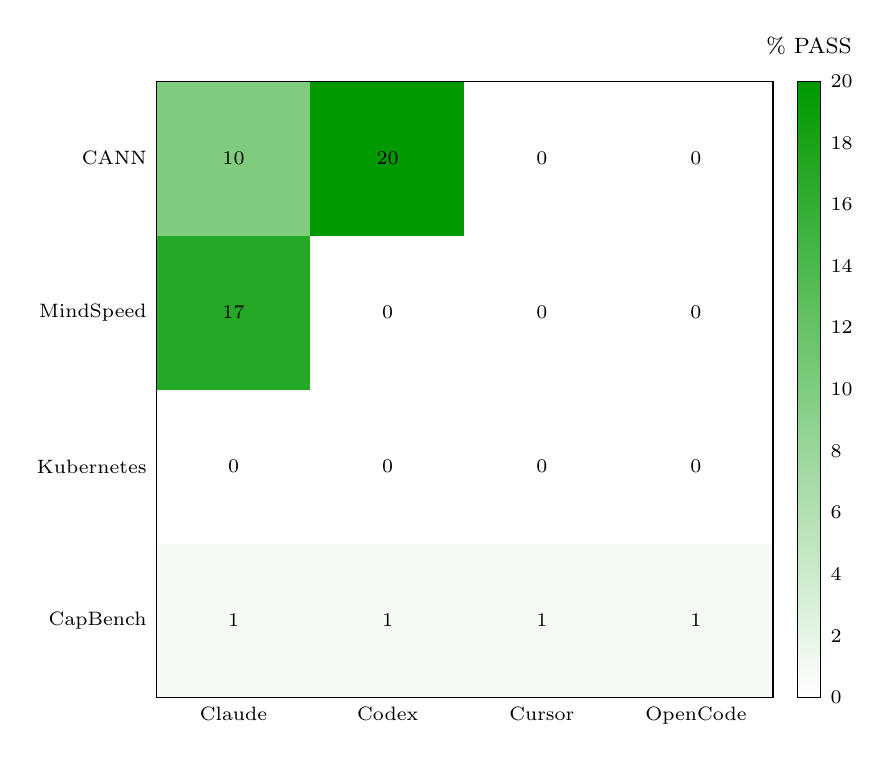
\begin{tikzpicture}
\begin{axis}[
    colormap={gr}{color=(white) color=(green!60!black)},
    colorbar,
    colorbar style={
      width=3mm,
      title={\footnotesize \% PASS},
      yticklabel style={font=\scriptsize},
    },
    point meta min=0, point meta max=20,
    xtick={0,1,2,3},
    xticklabels={Claude, Codex, Cursor, OpenCode},
    ytick={0,1,2,3},
    yticklabels={CapBench, Kubernetes, MindSpeed, CANN},
    tick style={draw=none},
    axis on top,
    enlargelimits=false,
    axis equal image,
    width=0.9\linewidth,
    xticklabel style={font=\scriptsize},
    yticklabel style={font=\scriptsize},
    nodes near coords,
    nodes near coords style={font=\scriptsize},
    nodes near coords align=center,
    point meta=explicit symbolic,
    every node near coord/.append style={yshift=0mm}
  ]
    \addplot[
      matrix plot*,
      mesh/cols=4,
      point meta=explicit,
      shader=flat corner,
    ] table[meta=v] {
      x y v
      0 0 1
      1 0 1
      2 0 1
      3 0 1
      0 1 0
      1 1 0
      2 1 0
      3 1 0
      0 2 17
      1 2 0
      2 2 0
      3 2 0
      0 3 10
      1 3 20
      2 3 0
      3 3 0
    };
  \end{axis}
  \end{tikzpicture}
  \caption{Pass rate (\%) by agent and task family under the majority-of-4 verdict. Rows top-to-bottom: \emph{CANN}, \emph{MindSpeed}, \emph{Kubernetes}, \emph{CapBench}. Kubernetes (K1--K4) is a \emph{uniform zero-pass} cliff across all agents.}
\label{fig:pass-heatmap}
\end{figure}


% Histogram of per-run mean score bucketed into 5 bins, one bar group per agent.
% Data derived from reports/eval_scores_v2_long.csv (mean of 4 evaluator composite scores per run).
% Buckets: [0,1), [1,2), [2,3), [3,4), [4,5]
\begin{figure}[t]
\centering
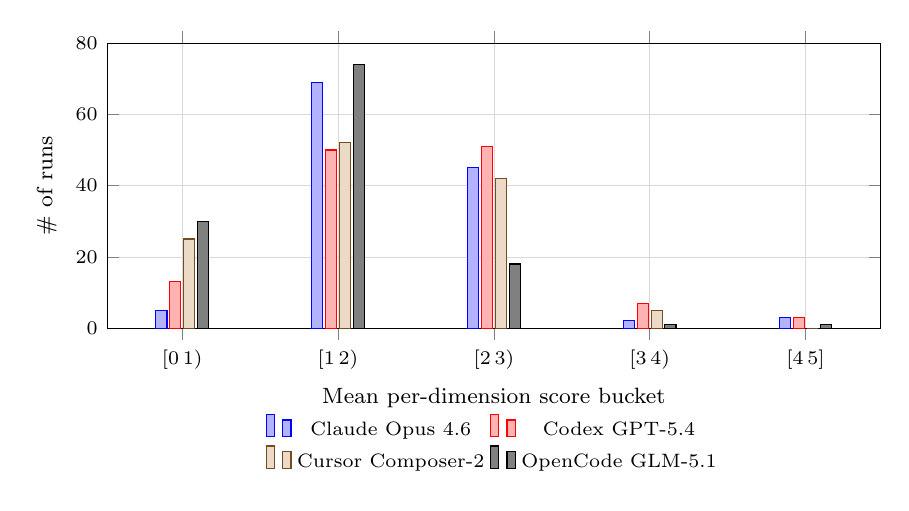
\begin{tikzpicture}
\begin{axis}[
  width=0.94\linewidth,
  height=5.2cm,
  ybar=1pt,
  bar width=4pt,
  symbolic x coords={[0\,1),[1\,2),[2\,3),[3\,4),[4\,5]},
  xtick=data,
  xlabel={\footnotesize Mean per-dimension score bucket},
  ylabel={\footnotesize \# of runs},
  ymin=0, ymax=80,
  enlarge x limits=0.12,
  legend style={font=\scriptsize, at={(0.5,-0.28)}, anchor=north, draw=none, legend columns=2},
  tick label style={font=\scriptsize},
  label style={font=\scriptsize},
  grid=both,
  major grid style={line width=0.2pt, draw=gray!30},
  minor tick num=0,
]
\addplot coordinates {([0\,1),5) ([1\,2),69) ([2\,3),45) ([3\,4),2) ([4\,5],3)};
\addplot coordinates {([0\,1),13) ([1\,2),50) ([2\,3),51) ([3\,4),7) ([4\,5],3)};
\addplot coordinates {([0\,1),25) ([1\,2),52) ([2\,3),42) ([3\,4),5) ([4\,5],0)};
\addplot coordinates {([0\,1),30) ([1\,2),74) ([2\,3),18) ([3\,4),1) ([4\,5],1)};
\legend{Claude Opus 4.6, Codex GPT-5.4, Cursor Composer-2, OpenCode GLM-5.1}
\end{axis}
\end{tikzpicture}
\caption{Per-run score distribution across four agents ($n{=}124$ runs each, combining 100 main-corpus and 24 calibration runs). Each bucket uses the mean per-dimension score, i.e., $(A+B+C)/3$ averaged across the four judges on a 0--5 scale; Table~\ref{tab:config-pass} reports the corresponding summed 0--15 composite mean. Most runs cluster in the 1--3 range, reflecting partial-pass behavior; full-rubric SE-PASS requires scores well above 4.}
\label{fig:score-histogram}
\end{figure}


%% ------------------------------------------------------------------
\subsection{Prompt Effect (Long vs Short)}
\label{sec:results-prompt}

Each of the 62 tasks was run with both a short ($\le 3$-sentence) and a long (detailed architectural spec) prompt. Table~\ref{tab:prompt} aggregates pass rates and mean scores by agent and prompt type.

\begin{table*}[t]
\caption{Prompt effect. $\Delta$ = long $-$ short, percentage points.}
\label{tab:prompt}
\centering
\small
\begin{tabular*}{\textwidth}{@{\extracolsep{\fill}}lrrrrrr@{}}
\toprule
\textbf{Agent} & \textbf{Short SE-PASS} & \textbf{Long SE-PASS} & \textbf{$\Delta$SE-PASS} & \textbf{Short mean} & \textbf{Long mean} & \textbf{$\Delta$mean} \\
\midrule
Claude   & 0.0\% & 4.8\% & +4.8 & 5.08 & 6.28 & +1.20 \\
Codex    & 0.0\% & 4.8\% & +4.8 & 5.20 & 6.44 & +1.24 \\
Cursor   & 0.0\% & 1.6\% & +1.6  & 4.00 & 5.77 & +1.77 \\
OpenCode & 0.0\% & 1.6\% & +1.6 & 3.72 & 4.60 & +0.88 \\
\bottomrule
\end{tabular*}
\end{table*}

On the main corpus, all four agents move from 0/50 short to 1/50 long SE-PASS, but the 1/50 is entirely T10. Excluding T10, long prompts improve mean composite score by +0.99 to +2.12 across agents but produce zero SE-PASS. The asymmetric SE-PASS lift visible in Table~\ref{tab:prompt} (Claude/Codex 4.8\% vs.\ Cursor/OpenCode 1.6\%) is a calibration-subset phenomenon: on the main corpus the prompt effect is uniform across agents.

\textbf{Finding 3:} Longer prompts help all four agents on mean score, but SE-PASS conversion occurs only on trivially-scoped (T10) or low-complexity calibration tasks. On the 49 non-trivially-scoped main-corpus tasks, detailed prompts improve partial quality without crossing the SE-PASS threshold. The asymmetric lift (Claude/Codex 4.8\% vs.\ Cursor/OpenCode 1.6\%) originates in the calibration subset where model capability interacts with bounded task scope.

%% ----------------------------------------------------------------
\subsection{Evaluator Agreement}
\label{sec:results-agreement}

Pairwise verdict agreement among the four evaluators spans from 42.5\% (Codex-GLM, the strictest pair) to 74.4\% (Claude-Cursor, the most aligned).

Codex and GLM agree the least (42.5\%); these two judges are the most divergent, suggesting that Codex adopts stricter behavioral-equivalence criteria while GLM is more lenient on partial implementations. Claude and Cursor agree most often (74.4\%). Full 4-way consensus occurs on 33.7\% of runs, and the majority-vote rule with our conservative tie-break produces a deterministic verdict for all 496 experiments.

\textbf{Finding 5.} Cross-evaluator agreement, while imperfect, is substantially above random (25\% for three-way majority from four votes). The 42.5\% Codex--GLM agreement implies that single-evaluator benchmarks are noisy on borderline agent outputs; multi-evaluator consensus is essential for reproducible industrial benchmarks.

%% ------------------------------------------------------------------
\subsection{Per-Task SE-PASS Distribution}
\label{sec:per-task}

Of the 62 tasks, only 4 have any SE-PASS across the 4 agents: C1, C4, M1, and T10. The rerun of disputed Cursor cases removes the previous C1-short, C4-short, and T34-long Cursor SE-PASS outcomes. Table~\ref{tab:task-pass-distribution} summarises the per-task SE-PASS distribution.

\begin{table*}[t]
\caption{Tasks that any agent reached SE-PASS (majority verdict across 4 judges) in at least one prompt variant.}
\label{tab:task-pass-distribution}
\centering
\small
\begin{tabularx}{\textwidth}{@{}lYr@{}}
\toprule
Task & Agents reaching SE-PASS (and prompt) & Total SE-PASS (of 8 runs) \\
\midrule
C1 (calibration) & Claude (long), Codex (long) & 2 \\
C4 (calibration) & Codex (long) & 1 \\
M1 (calibration) & Claude (long) & 1 \\
T10 (main corpus, trivially scoped) & Claude, Codex, Cursor, OpenCode (all long) & 4 \\
\midrule
\textbf{Total} & 8 / 496 & 1.6\% \\
\bottomrule
\end{tabularx}
\end{table*}

\textbf{Finding 4 (updated):} \emph{SE-PASS is concentrated in bounded tasks.} The 8 SE-PASS outcomes cluster in four tasks: three calibration tasks of low or localised scope (C1, C4, M1), and T10, the only trivially-scoped task in the main corpus (1 file, 482 diff lines). On the 49 non-trivially-scoped main-corpus tasks, no agent achieves any SE-PASS across 392 runs. Task complexity creates a near-absolute capability cliff: SE-PASS rate drops from 18.8\% on calibration Low tasks to 0\% on Medium tasks, and the CapBench aggregate of 1.0\% is entirely attributable to T10.

\iffalse
%% ----------------------------------------------------------------
\subsection{Statistical Robustness Checks}
\label{sec:results-stats}

To quantify how much of the pattern above survives choice of judge, choice of agent, and variance in task difficulty, we performed robustness checks on the full $1\,984$-verdict matrix.

\paragraph{Inter-evaluator agreement (Fleiss' $\kappa$).}
Overall 4-way Fleiss' $\kappa = 0.30$, corresponding to the \emph{fair} band on the Landis--Koch scale. Pairwise Cohen's $\kappa$ ranges from $0.13$ (Codex vs.\ GLM; the strictest and most lenient judge pair) to $0.51$ (Claude vs.\ Cursor). Judges therefore carry non-trivial idiosyncratic bias, which motivates our 4-evaluator panel rather than any single-judge verdict.

\paragraph{Judge-severity spread.}
Mean $A$-score (functional correctness, 0--5) ranges across evaluators from Codex $1.52$ to GLM $2.49$---a one-point gap on a 5-point scale. The strictest judge (Codex) marks $1.6\%$ of runs as SE-PASS; the most lenient (GLM) marks $4.0\%$. Absolute SE-PASS rates are thus judge-dependent; \textbf{only multi-evaluator consensus yields stable absolute numbers.}

\paragraph{Agent ranking is stable at the coarse level.}
Despite the severity spread, all four judges place Codex and Claude in the leading group and OpenCode in the trailing group by mean $A$-score. Cursor moves from the leading group to the lower group after the disputed Cursor reruns, which is precisely why we report both absolute SE-PASS counts and mean composite scores rather than a single leaderboard.

\paragraph{Prompt-length effect is statistically significant.}
Comparing long vs.\ short prompt variants (each task evaluated in both conditions), long prompts yield $3.2$\% SE-PASS across all 4 agents vs.\ $0.0$\% for short prompts. A $\chi^2$ test on the $2{\times}2$ pass/fail table gives $\chi^2 = 8.13$, $p = 0.004$. Long prompts also produce higher mean $A$/$B$/$C$ dimension scores by $+0.36$, $+0.52$, and $+0.39$, respectively.

\paragraph{Task-size determines feasibility.}
Across tasks, the Spearman rank correlation between GT diff size and SE-PASS rate is $\rho = -0.40$ ($p < 0.01$). Binning by GT-diff size:
\begin{center}
\begin{tabular*}{\columnwidth}{@{\extracolsep{\fill}}lr@{}}
\toprule
GT diff size (LOC) & Mean SE-PASS rate \\
\midrule
$< 100$       & $12.5\%$ \\
$100$--$500$  & $25.0\%$ \\
$500$--$2000$ & $1.0\%$ \\
$2000$--$10000$ & $0.0\%$ \\
$> 10000$     & $0.0\%$ \\
\bottomrule
\end{tabular*}
\end{center}
A logistic regression of SE-PASS on $\log_{10}(\text{GT LOC})$ alone yields a negative slope: larger required changes sharply reduce the odds of SE-PASS. This dominates all other covariates we measured and is consistent with the all-fail Kubernetes family.

\paragraph{Self-bias of evaluators.}
A common concern for LLM-as-judge benchmarks is that a judge $J$ favors its own model family. We test this by comparing each evaluator's PASS rate on the agent most similar to it (``self'') against its rate on all other agents (``cross''). The gaps are small relative to the overall failure rate: Claude ($4.0\%$ self vs.\ $2.4\%$ cross), Codex ($2.4\%$ vs.\ $1.3\%$), Cursor ($1.6\%$ vs.\ $2.7\%$), and GLM ($1.6\%$ vs.\ $4.8\%$). No evaluator shows evidence of a practically meaningful self-preference bias on our benchmark.

\textbf{Finding~6 (robustness).} The main conclusions survive the rerun of disputed Cursor cases.
\fi
